\documentclass{ctexart}
\usepackage{geometry}
\usepackage{fancyhdr}
\usepackage{graphicx}
\graphicspath{{./Qss/}{./}}
\usepackage{booktabs}
\usepackage{amsmath}
\usepackage{tikz}
\usepackage{array}
\xeCJKsetup{CJKmath=true} 
\usepackage{zhnumber} % change section number to chinese
\renewcommand\thesection{\zhnum{section}}
\renewcommand \thesubsection {\arabic{subsection}}
\CTEXsetup[format={\Large\bfseries}]{section}

\geometry{
    a4paper,
    left=3.18cm,
    right=3.18cm,
    top=3.04cm,
    bottom=3.04cm
}

\pagestyle{fancy}
\fancyhf{}
\renewcommand{\headrulewidth}{0.7pt} % 设置页眉横线粗细
\fancyhead[L]{\kaishu\large 大学物理实验报告} % 在左侧设置页眉文字
\fancyhead[R]{\kaishu\large 哈尔滨工业大学(深圳) } % 在右侧设置页眉文字
\fancyfoot[R]{\thepage} % 将页数放在右下角


\setlength\headwidth{\textwidth}

\begin{document}

\noindent
\textbf{
    \begin{tabular}{p{2.4cm}p{2.4cm}p{4cm}p{3.8cm}}
        班级 \hrulefill & 学号 \hrulefill & 姓名 \hrulefill & 教师签字 \hrulefill \\
    \end{tabular}\\
    \begin{tabular}{p{6cm}p{3.6cm}p{3.55cm}}
        \ 实验日期 \hrulefill & 预习成绩 \hrulefill & 总成绩 \hrulefill
    \end{tabular}\\
}
\rule[-10pt]{\textwidth}{0.7pt}

\begin{center}
    \Large \textbf{实验内容 \underline{准稳态法测不良导体的比热容和导热系数}}
\end{center}

\section{预习}
略

\newpage
\section{原始数据记录}
略

\begin{tikzpicture}[remember picture,overlay]
    \node[anchor=south east,inner sep=100pt] at (current page.south east) {
        \renewcommand{\arraystretch}{1.5} % 表格行高倍数
        \setlength{\tabcolsep}{18pt}    
    \begin{tabular}{|c|c|}
        \hline
        \LARGE  教师 & \LARGE  姓名 \\
        \hline
        \LARGE \kaishu 签字 &  \\
        \hline
        \end{tabular}
    };
\end{tikzpicture}

\newpage
\section*{三、数据处理}
\subsection{用 Origin 或其它程序画出加热面与中心面的 $T-\tau$ 曲线，以及 $\Delta T-\tau$ 曲线，从图上判断何
时进入准稳态，并求出 $\Delta T$ 及 $dT/d\tau$；}

本实验中，铜-康铜热电偶的温差电动势与其两端温度差呈线性关系，比例系数k为$40\mu V/K$。由此可以通过测量出的热电偶的电动势来计算$T$ 及 $\Delta T$。

通过Python程序绘制的$T-\tau$ 曲线和 $\Delta T-\tau$ 曲线如下所示：

\begin{figure}[htbp]
    \centering
    \begin{minipage}[t]{0.46\textwidth}
        \centering
        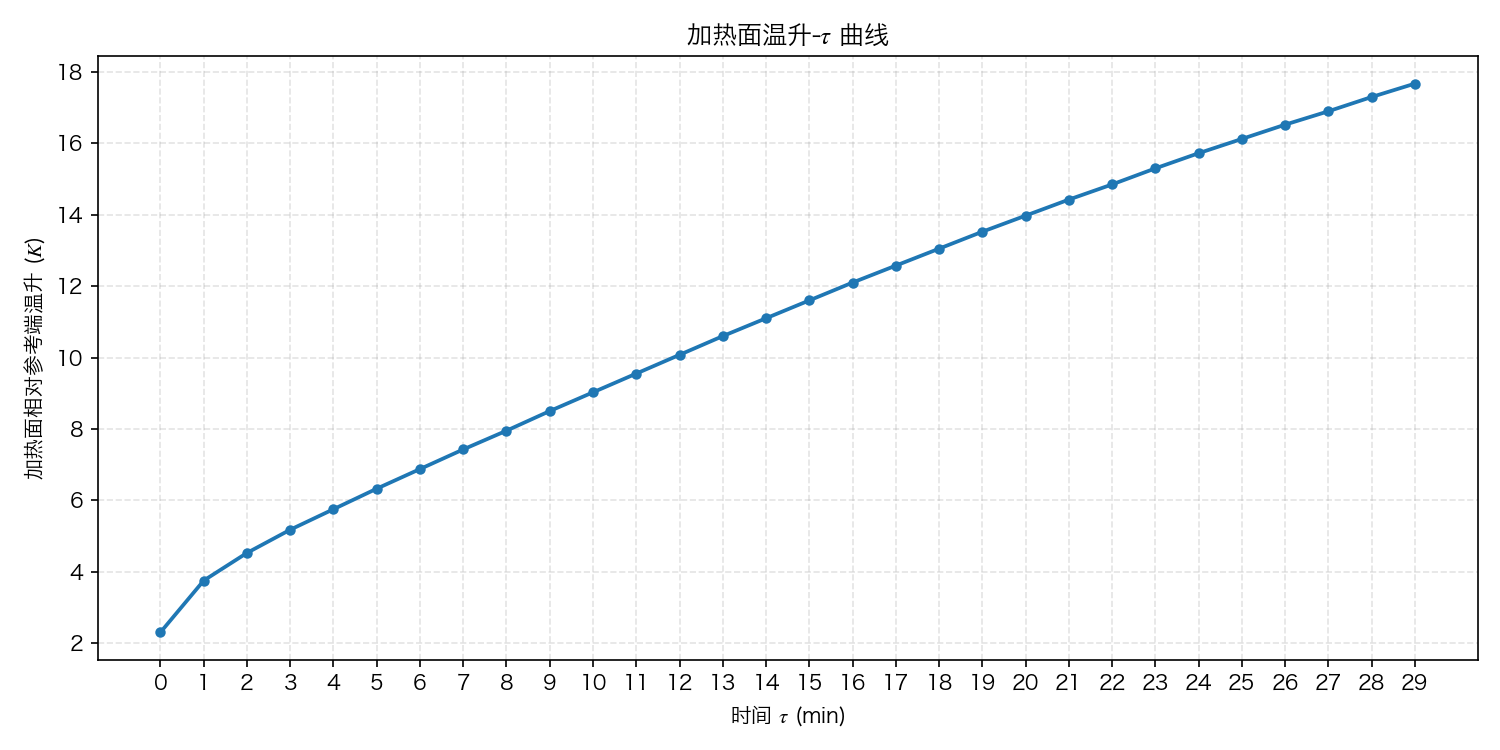
\includegraphics[width=\textwidth]{heat_curve.png}
        \par\vspace{0.4em}
        {\small （a）加热面相对参考端温升随时间变化曲线}
    \end{minipage}
    \hspace{0.04\textwidth}
    \begin{minipage}[t]{0.46\textwidth}
        \centering
        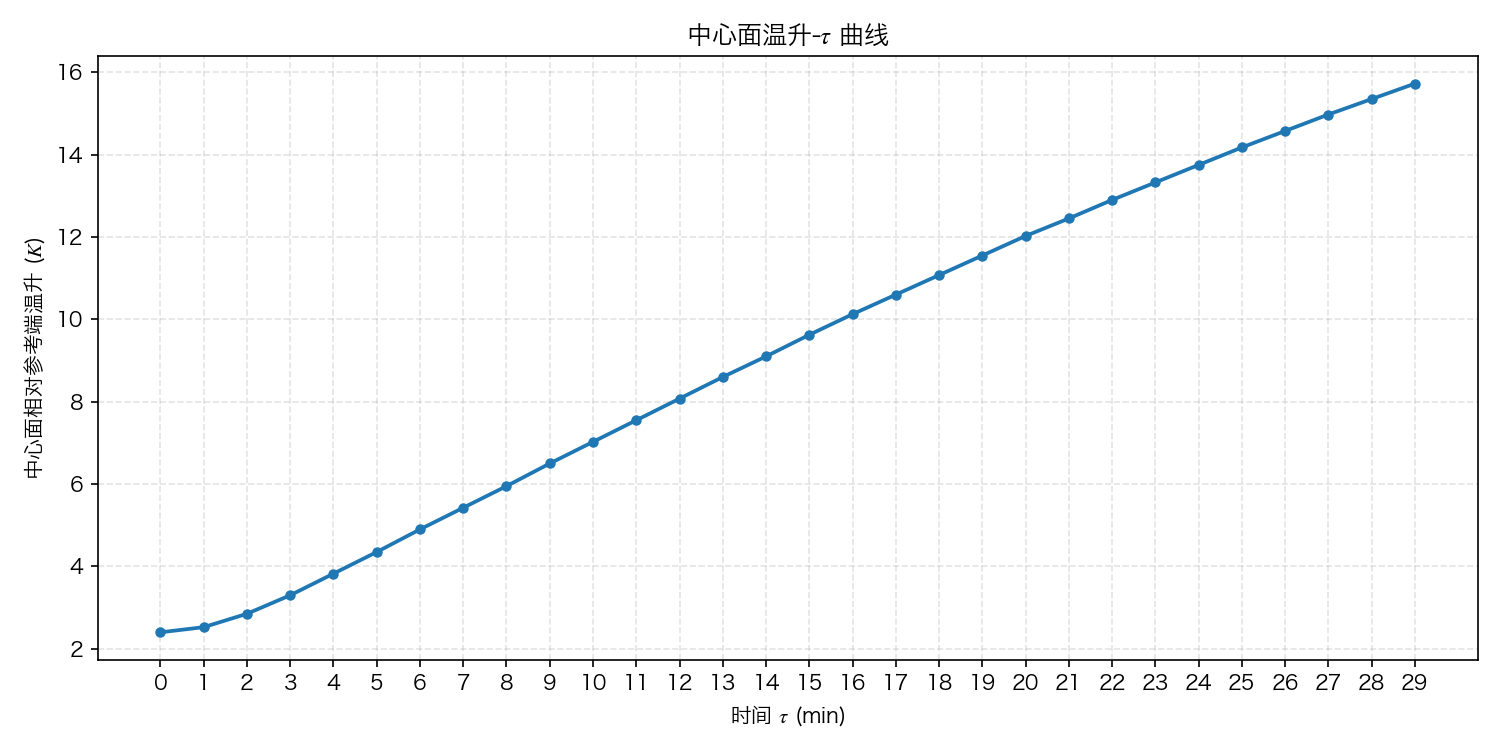
\includegraphics[width=\textwidth]{central_curve.png}
        \par\vspace{0.4em}
        {\small （b）中心面相对参考端温升随时间变化曲线}
    \end{minipage}
    \caption{加热面与中心面相对参考端温升随时间变化曲线}
\end{figure}

\begin{figure}[htbp]
    \centering
    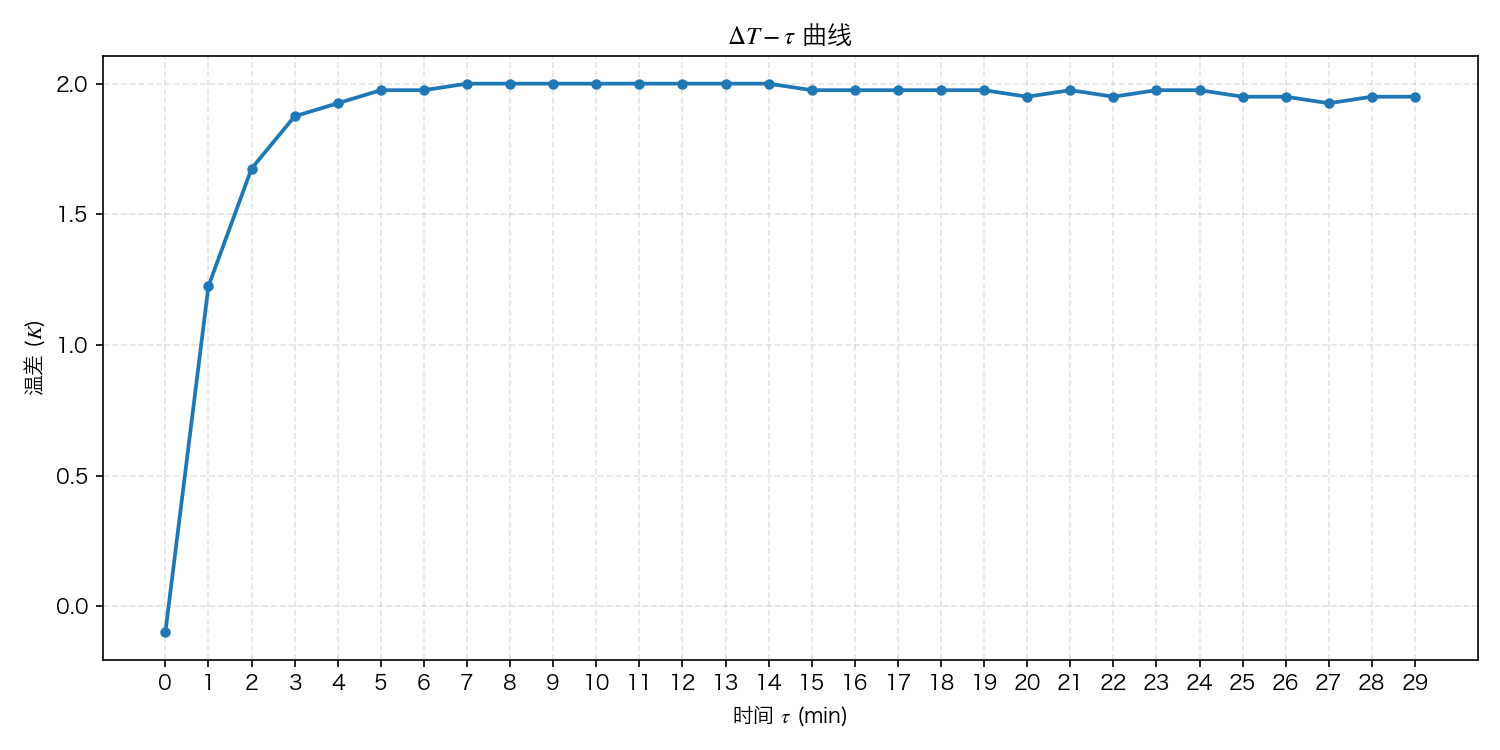
\includegraphics[width=0.88\textwidth]{heat_minus_central_curve.png}
    \caption{$\Delta T-\tau$ 曲线}
\end{figure}

由图可见，在 $\tau \approx 7\,\mathrm{min}$ 后，加热面与中心面的 $T-\tau$ 曲线近似为两条平行直线，且 $\Delta T-\tau$ 曲线基本保持稳定，因此可认为系统自此进入准稳态。

取准稳态区间为 $\tau=7\sim14\,\mathrm{min}$，根据最小二乘法，可得：
\[
\Delta T \approx 2.00K,
\qquad
\frac{dT}{d\tau} \approx 0.53\,K/min.
\]


\subsection{计算有机玻璃样品和橡胶样品的导热系数和比热容。}

实验中只测了橡胶样品的数据，因此只计算橡胶样品的导热系数和比热容。

根据准稳态法的原理，导热系数 $\lambda$ 和比热容 $c$ 可以通过以下公式计算：
\[
\lambda = \frac{q_c R}{2 \Delta T},
\quad
c = \frac{q_c}{\rho R \frac{dT}{d\tau}},
\]

其中，样品材料的密度$\rho=1304\,\mathrm{kg/m^3}$，平板厚度的一半$R=0.01\,\mathrm{m}$，热流密度$q_c=\frac{AV^2}{2Fr}=\frac{0.85 \times 18.00^2}{2 \times 0.09^2 \times 115.25}= 147.50\,\mathrm{J/(m^2 \cdot s)}$。代入上述公式计算可得：

\[
\lambda \approx 0.37\,\mathrm{W/(m\cdot K)},
\qquad
c \approx 1280\,\mathrm{J/(kg\cdot K)}.
\]

\section*{四、实验现象分析及结论}

加热7分钟后， 中心面温度和加热面温度近似呈线性变化，加热面和中心面的温差基本保持不变，橡胶样品进入准稳态。测得橡胶样品的导热系数和比热容分别为：

\[
\lambda \approx 0.37\,\mathrm{W/(m\cdot K)},
\qquad
c \approx 1280\,\mathrm{J/(kg\cdot K)}.
\]

\section*{五、讨论题}

\subsection*{1. 本实验中我们采取在样品两端加热的方式根据加热面与中心面的温差及端面温升速率求出导热系数和比热。实验中为何使用四块样品？}

因为加热膜发出的热量是向两面传导的，所以这样的对称结构可以保证向样品传导的热流占加热器电功率的一半；同时可减小边缘散热影响，从而使得热流密度的计算更为方便、准确。

\subsection*{2. 本实验中判断系统进入准稳态的条件是什么？}

\begin{itemize}
    \item 加热面与中心面的 $T-\tau$ 曲线近似为两条平行直线；
    \item $\Delta T-\tau$ 曲线基本保持稳定。
\end{itemize}

\subsection*{3. 本实验中准稳态会无限保持下去吗？是否时间越长实验数据越好？}

准稳态不会无限保持下去，也不是加热时间越长实验数据越好。

随着加热时间延长，样品与环境的温差增大，散热损失等影响会逐渐增强，系统将逐步偏离理想准稳态条件，使加热面与中心面的升温速率不再严格相同，$\Delta T$ 也会发生变化，故延长测量时间对实验无益。

\end{document}
